\section{Introduction}
Our purpose is to find a solution that will automate the reduction of ULTRACAM objects. In this chapter we outline our approach and some of the difficulties we have encountered. 

In recent years several projects for automated sky observations have been launched, the Monitor project \citep{Irwin2007} , the Catalina survey \citep{CatalinaCatalog}, the WASP project \citep{PollaccoSuperWASP} and the Hungarian Automated Telescope (HAT) \citep{BakosHATNet} are just a few examples. More are planned in future with the most notable being the Large Synoptic Survey Telescope \citep{lsst}. All of these surveys use automated reduction pipelines. Some of the techniques they are using can be applied to non-automated observations such as ULTRACAM runs. However, since these runs are non-automated, we will need to address various difficulties that arise. The advantage that automated observations have is that the reduction pipeline is able to make several assumptions about the data it is reducing. It can usually rely on consistent image size, field scale and orientation. Automated surveys generally have the same exposure times and cadences throughout their measurements. Since our data source is from non-automated observations, our pipeline needs to be able to cope with a wide range of these parameters. An example of one of these challenges is finding astrometric solutions to our fields. Since the ULTRACAM fields vary widely in how that are windowed (see figures \ref{fig:KOI-824} to \ref{fig:V834Cen}), these data do not have regular images of the sky and could be missing large fractions of the image, making astrometric solutions difficult in many cases. We describe our approach to dealing with this diverse data set in this chapter. 

\section{Data reduction for CCD images in Astronomy}
Since the late 1980's, Charge Coupled Devices (CCDs) have risen to prominence in astronomy. Before CCDs, high-speed optical photometry was performed using photomultiplier tubes. Photomultipliers are high tension (high voltage) devices that detect faint light by using the photoelectric effect followed by amplification. When a photon impinges on the detector, an electron is ejected. This electron is then amplified by a series of voltage steps until the resulting signal is read out by an analog to digital convertor. The main problem with this configuration is that the photomultiplier only has one detection element and the light from the star needs to pass through a physical aperture in the instrument so that only light from the target object is measured. Using a single photomultiplier, it is not possible to measure multiple objects simultaneously. 

CCDs are 2-dimensional detectors covered with light sensitive semi-conductors (each one defining a `pixel') that are able to measure and count photons. The structure and construction of CCDs depends on their intended purpose. Consumer electronic devices such as the cameras in mobile phones or digital cameras use a different arrangement and read-out process to that used in astronomical CCDs. In order to decrease read-out times, consumer devices use an architecture called `interline' where the read-out pixels and electronics are located in alternate rows of the CCD. This means that every alternate row of the CCD is masked from light and used for readout only. The disadvantage of this architecture is that the fill-factor or area that is sensitive to light of the CCD is now reduced to 50\%. Astronomy purpose CCDs do not use inter-line pixels and do not mask any part of the imaging area.  The fill-factor of the astronomical CCDs is closer to 100\% as none of the pixels are masked. There is still a small gap between pixels though so we do not quite reach a fill-factor of 100\%. They read out the entire chip line-by-line and pixel-by-pixel before the next exposure can begin. This architecture has the advantage that it allows more time for the read-out process to take place. A slower read out process introduces less noise into the output. Slow readout is a problem if there is a requirement for high-cadence exposures as in ULTRACAM. For higher frame rates full-frame transfer devices are used. These devices are CCDs that are divided into 2 equal areas. One half of the device is exposed to light and the other half is masked. After each exposure, the exposed (or imaging) area is shifted completely into the masked (or storage) area. The imaging area is now ready to be exposed again, while the stored image can be read out from the storage area.  

CCDs can be sensitive to optical, infra-red and ultraviolet light depending on the materials used and their manufacture. In ULTRACAM, all three of the CCDs are E2V 47-20 CCDs. They are frame-transfer chips with imaging areas of 1024$\times$1024 pixels and storage areas of 1024$\times$1033 pixels.  To improve quantum efficiency, the ULTRACAM chips are thinned, back-illuminated and antireflection coated with E2V's enhanced broad-band astronomy coating (in the case of the blue and green chips) and standard mid-band coating (in the case of the red chip), \citep{dhillon07}.

Since the CCD is recording a 2-dimensional image of the sky, it will capture multiple objects simultaneously. In the 2-dimensional image it is possible to create a virtual aperture as part of the reduction process. Physical apertures (used with photomultipliers) needed to be large enough to account for changes in seeing and drifts in the target object's position as the telescope tracks the sky. Large apertures are a problem since the sky starts to contribute a significant amount of the total flux in the aperture. Nights with poor seeing and variable sky conditions were often not photometric in the days of photomultipliers. Nowadays, thanks to the nature of the CCD imaging, we can still get photometric data from nights with less than ideal seeing and variable atmospheric transmission.  Although early CCDs lacked the quantum efficiency of photomultipliers, this limitation has since been surpassed. Photomultipliers are rarely used nowadays, at least for optical astronomy. They are still used to detect photons from scintillations in Cerenkov detectors and neutrino detectors.  

In order to extract photometry from a CCD image, several steps are performed to convert the 2-dimensional image into a 1-dimensional flux measurement for each object in the image. This is known as reduction. Reduction in CCD photometry can be summarised as follows: 

\subsubsection{Bias subtraction:}
CCDs have an intrinsic noise known as readout noise. In order to ensure that this noise does not fluctuate around the value zero with the potential therefore of having a negative number in the output an arbitrary bias is set to ensure that each pixel always reads out a positive value. Since the pixel ADU values are stored as 16-bit unsigned integers, negative numbers would appear as large ADU values ($65535 - \mbox{value}$). During the night, bias frames are recorded by taking CCD readings without exposing the CCD to any light. These bias frames are then subtracted from each science CCD frame. 

\subsubsection{Flat fields:}
It is not certain that each pixel in the CCD array has the same sensitivity to light as its neighbours. This is a problem when trying to measure the flux of an object very accurately. If the object's light falls on different pixels in each subsequent exposure, then the pixel sensitivity will impact the measurement of the object's true flux. To measure each pixel's relative sensitivity, the entire imaging area is exposed to a uniform source. The source is either a white screen mounted on the inside of the dome, or, more commonly, an exposure of the sky during twilight. This flat-field is then normalised by dividing each pixel's count by the average of all the pixels. Each pixel's sensitivity can then be factored into our reduction of a science run. 

\subsubsection{Source extraction \& aperture creation:}
The exposed 2-dimensional image can have many sources on it and a method is needed to pick out the objects of scientific interest. Spurious image artifacts such as those caused by cosmic rays should be ignored. Source detection can be automatic, as we will use in this project, or manual, as performed with the current ULTRACAM reduction pipeline. The source extraction stage will produce a list of apertures. The apertures are defined by having a position (usually the centroid of the object) and a 2-dimensional area, which is usually a circle centred on the object's position that captures all the light from the object but excludes light from any other nearby objects. These apertures are virtual, defined in $(x, y, radius)$ parameter space, rather than physical as in the earlier photomultiplier devices. In this project, we will be using {SExtractor}, a popular, third party software package to perform the source extraction and aperture definition, (\citep{bertin}).

\subsubsection{Sky subtraction \& Flux measurement:}
The Earth's atmosphere is not completely dark at night and still glows blue with light scattered from the stars, reflected from the Earth or scattered from the Moon. This sky background needs to be taken into account and subtracted from the total flux measured in the aperture in order to leave the flux that is contributed by the target object. There are two main methods of dealing with the sky background. The first is to derive an overall sky-background for the image, which is then subtracted from the flux measured in the aperture. The flux remaining is then the flux contributed by the target object. This overall sky background is not a single value, but a polynomial fit in order to allow for smooth variations across the field. 

The second approach is to measure the flux in an annular aperture centred around the target object that is close enough to the object to have a similar sky reading, but also far enough away to ensure that no significant flux is contributed by the object itself. The flux per unit pixel in the annulus is subtracted from the flux per unit pixel in the object's aperture in order to remove the sky background. Calculating the size of the aperture and the inner radius of the annulus is aided by fitting a Moffat profile to the star's point-spread-function (PSF). The PSF is the two dimensional profile of the image as recorded on the CCD.  Either a Moffat profile or a Gaussian profile could be fit to match the PSF, but the Moffat profile is favoured as its shape matches the real PSF of the star's image since it was derived by convolving atmospheric seeing profiles with telescope diffraction profiles, \citep{Moffat69}. The formula for the Moffat profile is \begin{equation} I_r = I_0 {[1 + {(\frac{r}{\theta})}^2]}^{-\beta}\end{equation} where $I_0$ is the intensity at image center, $\theta$ is the half width at half maximum of the image in the absence of atmospheric scattering and $\beta$ is the atmospheric scattering coefficient. By fitting a Moffat profile to the star's PSF we can derive a value for the full width at half maximum (FWHM),  $2\theta$, of the star's image. This value gives a value to use to set the radius of the aperture and the inner and outer radii of the sky annular aperture. These values are generally pre-defined constants multiplied by the FWHM. The optimal value for the object aperture size is approximately 1.5 times the FWHM value, \citep{optimalapertures}.

\section{Current method of ULTRACAM data reduction}
Tom Marsh at the University of Warwick has developed a set of software tools for reduction of these ULTRACAM data. For the rest of this document we will refer to this pipeline as the \emph{traditional} pipeline and the new pipeline created in this project as the \emph{automated} pipeline. 

It is possible to run the traditional pipeline at the telescope during the observation. This allows observers to review these data live at the telescope. It also acts as a preview for the observer and allows adjustments to be made during the run. After the run, the raw data are copied to the archive and can be used for reduction later. This can happen the following day, or much later, when the observer has returned from the observatory. Any of these data in the data archive can be re-reduced at any time since all the raw data are stored. 

\begin{figure}
\centering
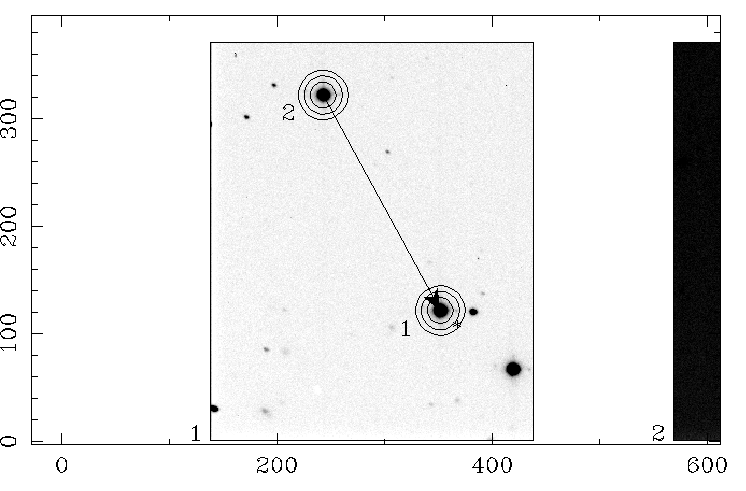
\includegraphics[width=110mm]{images/setaper.png}
\caption{Defining the apertures for the reduction using the \emph{traditional} pipeline. Note that the two apertures can be linked. This instructs the pipeline to maintain the pixel separation of the apertures even if there is a small amount of movement from frame to frame. This is useful if our target object is likely to fade significantly during the run.}
\label{fig:settingapertures}
\end{figure}

The current data reduction process for ULTRACAM is designed to produce three colour light-curves from the raw image data. The pipeline consists of the following stages:
\begin{enumerate}
	\item Producing bias frames that are used the calibrate the CCD detector's thermal noise characteristics. 
	\item Producing flat-fields to calibrate the pixel sensitivity of each of the 3 CCD detectors. 
	\item Defining apertures for the objects of interest in the run. This step involves manually choosing the objects of interest in the frames and defining the aperture sizes and positions for each object. Apertures are set independently for each channel (r, g, b). An example of this can be seen in figure \ref{fig:settingapertures}.
	\item Running the reduction software. The reduction code uses the apertures defined in the previous step and measures the flux of each object in each colour. The software is able to track changes in the object's size and shape due to changes in the point spread function (PSF) by scaling the virtual aperture. It is also able to track small changes in the positions of the objects. 
\end{enumerate} 

Although this process is not particularly cumbersome, it includes manual steps and it does not scale well when there are a large number of runs to be processed or if there are many target objects in a run. For example, the run shown in figure \ref{fig:KOI-824} contains more than 1000 objects. Manually defining apertures for each of these objects in each channel is not practical. An automated method would enable data reduction for all of the objects captured in each run without the need for manual intervention. 

\section{Automating the pipeline}
The outcome of this MSc project is a system that is able to process the raw image data from ULTRACAM and, without any manual intervention, produce a set of light-curves for all of the objects in the data. It produces a set of web pages that can be viewed from anywhere with an internet connection. 

\subsection{Algorithm of the automated pipeline} 
The following section describes the key steps in the automated pipeline at a high level. The subsequent sections will describe each in more detail:

\subsubsection{Key stages for automation}

\begin{figure}
	\centering
	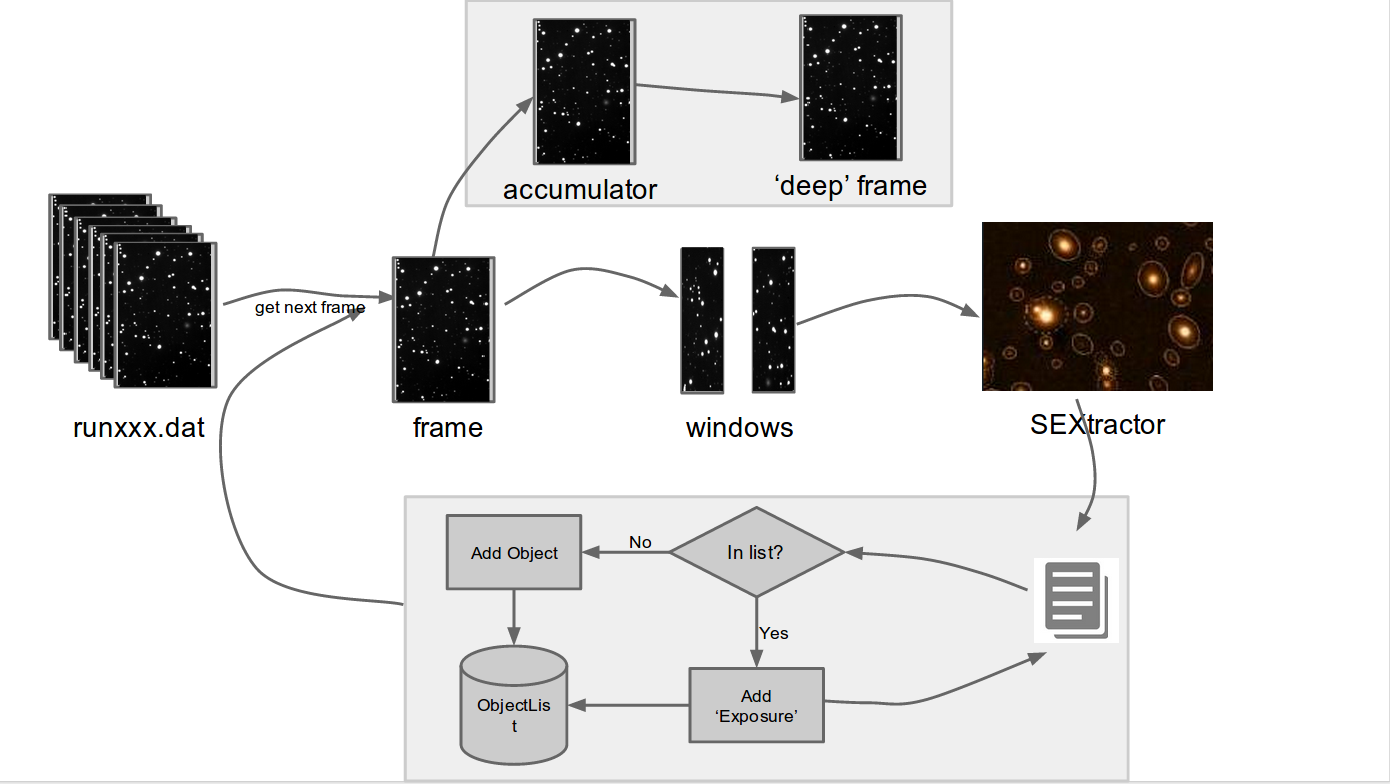
\includegraphics[width=130mm]{images/flowchart.png}
	\caption{Schematic of Stage 1 of the pipeline.}
	\label{flowchart}
\end{figure}

\begin{figure}
	\centering
	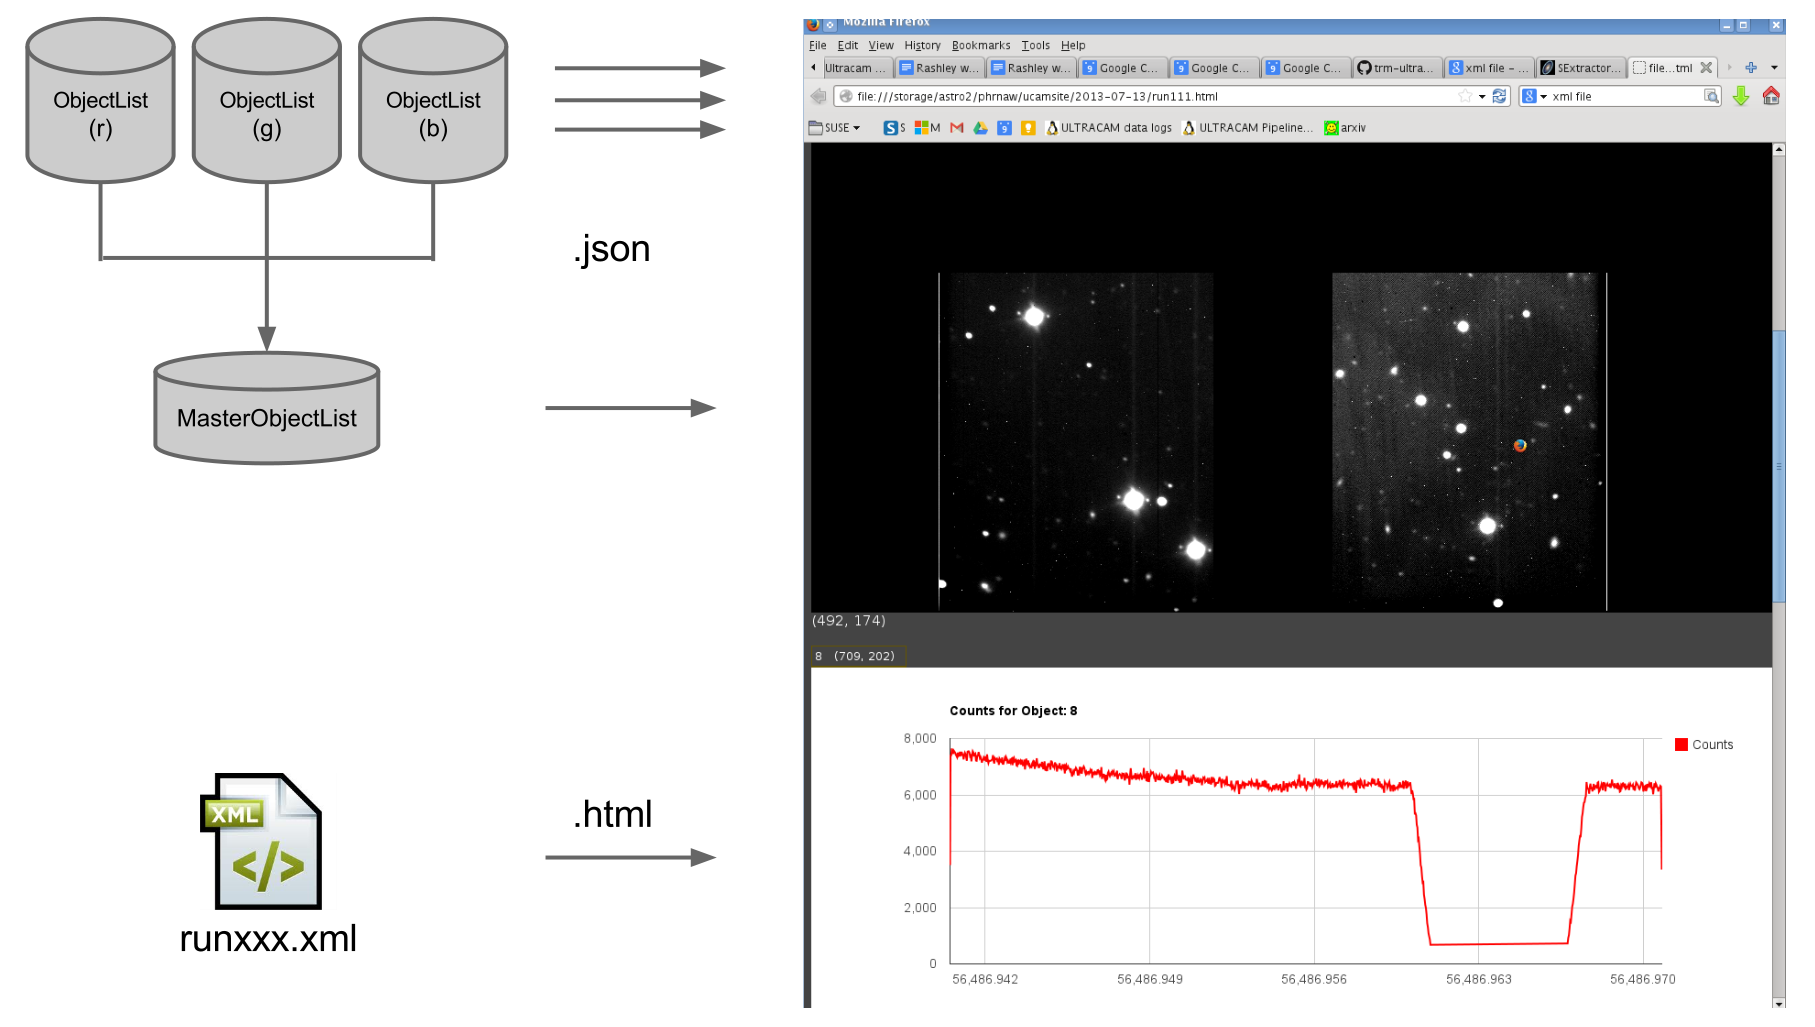
\includegraphics[width=130mm]{images/webpublish.png}
	\caption{Schematic of Stage 6 and 7 of the pipeline.}
	\label{webpublish}
\end{figure}

The stages of the reduction process are as follows:
\begin{enumerate}
	\item Extract all of the detectable objects in all of the frames. 
	\begin{enumerate}
		\item Read the raw image file, containing all frames for a particular run.
		\item Initialise an empty list of objects, called a catalog.
		\item For each frame in the run
		\begin{enumerate}
			\item For each colour channel in the frame.
			\item Extract each window from the frame.
			\item Send the window bitmap data to the SExtractor software.
			\item Use SExtractor to process these data and produce a catalog of all sources, with their positions and flux measurements.
			\item Read the results of the source extraction process, including pixel position and flux measurements for each object.
			\item For each object returned:
			\begin{enumerate} 
				\item Try to match this object with one already in the catalog, based on nearest distance.
				\item If the object is not already in the catalog, add it to the catalog as a new object.
			\end{enumerate}
		\end{enumerate}
		\item Store the list of objects for each of the three channels.
	\end{enumerate}
	\item Filter each catalog, removing objects that are likely to be artifacts. This is done by looking for objects that do not persist across more than a pre-defined percentage of frames; and objects that have a size equal to one pixel. 
	\item Sort the catalogs ordered by brightness as measured by the average flux. Pass these catalogs to the \emph{Astrometry.net} library to resolve the WCS solution for the fields. Perform this task separately for each of the three channels (r, g, b). Since each channel has a very slightly different view of the field and different distortions in the image, their respective WCS solutions will differ by a small amount.
	\item Merge the three catalogs by cross-identifying each object in each of the three channels. This may seem to be a trivial step for many ULTRACAM runs because the differences in the fields from channel to channel are minor, however in crowded fields such as the one shown in figure \ref{fig:KOI-824}, simply matching objects based on their pixel coordinates is not enough to disambiguate them.
	\item Produce deep images for each channel and export it to a web-viewable format, such as the Portable Network Graphics (PNG) format. 
	\item Create Javascript Object Notation (JSON) files and HTML files to enable the reduced data to be loaded into a web browser.
	\item Publish this `web-enabled' version of the information to a web site that is accessible outside of the university network.  
\end{enumerate}

\subsubsection{Source extraction}
A popular software tool used for source extraction is \emph{SExtractor}, \citep{bertin}. SExtractor is able to process a 2-dimensional image and produce a catalog of sources in that image, along with a measurement of the flux of each object. 

For each frame in the data run (which could consist of a few frames up to several thousand frames), the pipeline extracts the image data, which consists of a 2D pixel map with the CCD counts or analogue digital unit (ADU) for each pixel, and passes this to SExtractor for source extraction. 

SExtractor performs two passes on this image. On the first pass it makes an estimate of the background signal of the entire image. It assumes that the background-signal contains both the sky-background and the bias of the CCDs as the pipeline has not subtracted the bias from each frame before passing it to SExtractor. It estimates the background by creating a mesh-grid of background readings for the whole image, applying a median clipping algorithm and then fitting a bicubic spline to interpolate between the mesh points. It then subtracts this background from the image. The size of the mesh grid is configurable and the pipeline allows the user to tweak this parameter if necessary. In the current version of the pipeline, this parameter is not configured automatically.  If small scale changes in the background are expected then the mesh size should be reduced. The usual value used in the pipeline is a mesh grid size of 64 pixels. It appears that this setting is suitable for all runs in the ULTRACAM archive as there has been no obvious need to adjust this parameter so far. 

On the second pass, SExtractor applies a convolution filter to the image. This step is intended to increase the detectability (enhance the signal-to-noise ratio) for target objects on the frame. The default filter used in the pipeline is a simple `circular' PSF defined by the 3x3 mask\footnote{This filter is normalised before being applied to the image.}:
\[
\begin{array}{ccc}
  1 & 2 & 1 \\
  2 & 4 & 2 \\
  1 & 2 & 1 \\
\end{array}  
\]

SExtractor then applies thresholding to the background subtracted and filtered image. The threshold for detection is defined as the pixel's ADU value above the background (in units of the background's standard deviation). This threshold is configurable and can be modified before running the automated pipeline. The default value used for most of the pipeline processing is $3\sigma$. Decreasing this parameter will have the effect of increasing the number of objects detected for any particular run. Reducing it too much will cause the source extraction to produce many spurious object detections. For example, setting this value to $1\sigma$ results in the source extraction identifying spurious sources that are really just noise in the background. This leads to the automated pipeline being overloaded with too many new sources to process, causing it to grind to a halt as the number of tracked objects climbs rapidly. At the moment, the automated pipeline is not able to automatically tune this parameter for each run, although this is something that will be considered for future iterations of the software. Figure \ref{fig:tweakingthreshold} shows how modifying this threshold parameter can increase the number of objects detected by the pipeline.

The image in figure \ref{fig:tweakingthreshold} has been created by stacking all of the images in the sequence, consisting of 726 frames. Stacking reveals objects that are not visible above the noise when analysing each individual frame. Since the pipeline extracts sources for each frame in turn, it is not able to detect these fainter objects that are so clearly revealed on the deep, stacked images. This suggests that, for future iterations of the pipeline, a different approach might be taken for source extraction and aperture definition. One idea is to perform a first pass to produce a stacked image and then use this image for source detection and aperture creation. These pre-defined apertures would then be used as an input for the flux measurement of each frame. This approach would need some flexibility in order to be able to deal with small movements of the objects from frame to frame and to enable aperture tracking of objects that move through the field (such as asteroids).

\begin{figure}
  \centering
  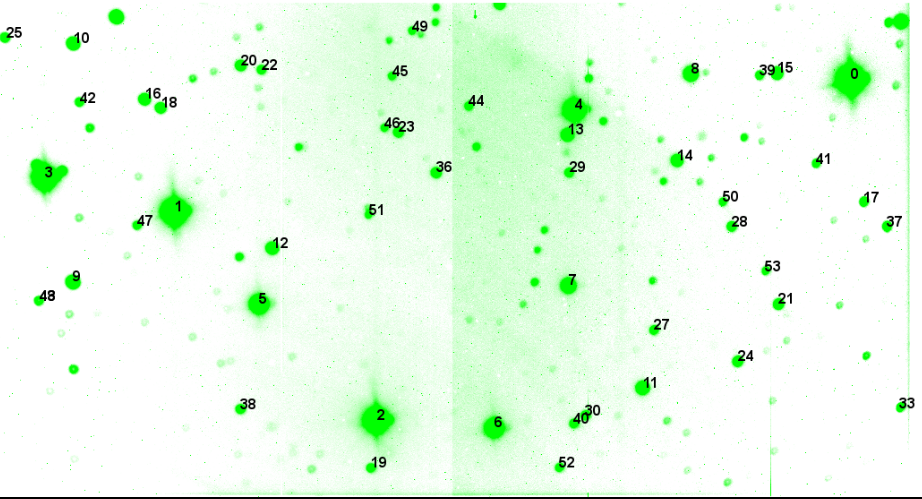
\includegraphics[width=.8\linewidth]{images/2012-09-03_g_default.png}
  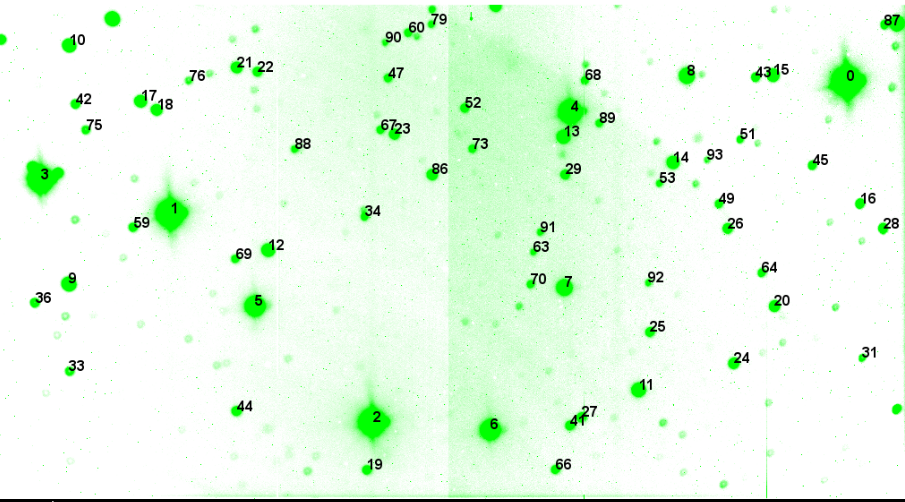
\includegraphics[width=.8\linewidth]{images/2012-09-03_g_15sigma.png}
  \caption{The effect of tweaking the DETECT\textunderscore THRESH parameter in SExtractor. The upper plot shows the objects detected in a run with the threshold set at $ 3\times \sigma_{background}$ [56 objects detected], while the lower plot was produced with DETECT\textunderscore THRESH set at $ 1.5\times \sigma_{background}$  [101 objects detected]. Note: setting it to 1.2 detected 149 objects, but slowed the processing of the entire run by a factor of 3x. }
\label{fig:tweakingthreshold}
\end{figure}

SExtractor then determines the pixel position of each object by calculating a weighted mean in the $x$ and $y$ dimensions. The weighting applied to each pixel is the pixel intensity (after background subtraction and filtering). If $I_{i}$ is the pixel intensity for pixel $i$ in the segmented collection of pixels, then: \begin{equation}\bar{x} = \frac{\sum\ I_{i}x_{i}}{\sum I_i}\end{equation} and \begin{equation}\bar{y} = \frac{\sum\ I_{i}y_{i}}{\sum I_i}\end{equation}

\subsubsection{Flux measurement}
For each object that has been selected through the threshold criterion, the flux is then calculated. This is computed by one of 2 methods. 

\emph{AUTO: Automatic aperture mode}
SExtractor uses a routine inspired by Kron's `first moment' algorithm, \citep{kron}. It defines an elliptical aperture that has an elongation $\epsilon$ and position angle $\theta$ defined by the second order moments of the object's light distribution. Across this ellipse, a first moment is computed $r_1 = \frac{\sum r I_r}{\sum{I_r}}$. The aperture is then scaled by user defined parameters to 2.5-3.5 times $r_1$. This scale factor is configurable by the user before the run, but does not require modification for this project. 

\emph{APER: Fixed aperture mode}
In this mode, the measurement of flux for the object is calculated by summing the background subtracted pixel intensity, $I_{x,y}$,  of all of the pixels that are within a pre-defined aperture radius centred on the $x, y$ position as calculated above. SExtractor does not perform a Moffat fit to the PSF.  Flux is then given by, \begin{equation}F = \sum\limits_{x,y \in aperture}I_{x,y}\end{equation}

When using the fixed aperture mode, the aperture radius is defined before the pipeline is run and is specified manually. Due to the diversity of data in the ULTRACAM archive, there is no obvious single choice for this value. For example, some of the runs containing bright sources (ie magnitude 12 and brighter) that are follow-up observations of sources found in the {SuperWASP}\footnote{\url{http://www.superwasp.org/}}, \citep{PollaccoSuperWASP} and {HAT}\footnote{\url{http://hatnet.org/}}, \citep{BakosHATNet}, surveys use the telescope in a deliberately de-focused state. De-focussing the telescope to this extent transforms the Moffat-like PSF into something that resembles a flat disc, or even, in extreme cases, a disc with a hole in the centre (which is an image of the secondary mirror). In this case, the fact that SExtractor does not attempt a Moffat fit is an advantage. Aperture sizes for these runs need to be between 50 and 80 pixels. When the telescope is in focus however, far smaller apertures of between 8 and 15 pixels are needed. It is conceivable that the decision on what aperture size could be automated by the new pipeline. A simple way to do this would be to perform a 2-pass approach. First use AUTO aperture mode to have SExtractor return a list of aperture sizes, then choose a fixed aperture size that represents the best choice for this run, most likely the median of the aperture sizes returned after the first-pass. This is something that will be considered for future iterations of the pipeline. 

\begin{figure}
  \centering
  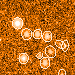
\includegraphics[width=50mm]{images/sex_apertures_auto_cropped.png}
  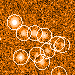
\includegraphics[width=50mm]{images/sex_apertures_fixed_cropped.png}
  \caption{AUTO vs FIXED apertures in SExtractor. The image on the left is the result of using the AUTO aperture setting in SExtractor. Note that apertures can be elliptical and are allowed to overlap. On the right is a FIXED aperture setting with the aperture diameter set (manually) to 15 pixels. The FIXED aperture is always circular.}
\label{fig:fixedautoapertures}
\end{figure}

In order to facilitate the automatic running of the pipeline across the entire ULTRACAM data archive, the default setting for the flux measurement is the AUTO aperture mode. This means that SExtractor uses the algorithm described above to determine the most appropriate aperture size for each object. After inspection of the output, runs that would benefit from fixed apertures can then be re-computed with a manual setting for the aperture size. 

The output from SExtractor is a FITS file that contains a catalog of all of the detected objects with measurements of their flux. Each individual window of each frame in each channel (r, g, b) are treated separately by SExtractor and there is no tracking of objects. The catalog returned by SExtractor doesn't maintain a list of object identifiers (IDs) that are consistent from frame to frame. Since the source extraction is performed for each frame individually, the ranking of the objects may change and some fainter objects may not appear in each returned catalog. The task of building and maintaining a consistent list of the objects is undertaken by the automated pipeline software built for this project. 

\subsubsection{Object tracking}
The automated pipeline creates light-curves for all of the objects and, in order to do so, it needs to keep track of these objects throughout the run (across frames and channels). The approach is to use the pixel $(x, y)$ coordinates of the objects returned by SExtractor as the key attribute for identifying an object that recurs from frame to frame. For each window sent to SExtractor, the pipeline performs the following steps:
\begin{enumerate}
  \item{Read} the catalog file, containing the $(x, y)$ coordinates and fluxes for all objects in the window.
  \item{Rank} all of the objects from brightest to faintest.
  \item{Transform} the pixel coordinates from the reference frame of the individual window, to an overall reference frame, matching the size of the full CCD. 
  \item{Match} all objects in the catalog. For each object in the list, check its proximity to any objects that have been identified on previous frames. The distance threshold for a match is configurable and the default is 10 pixels. If there is more than one match, the closest match wins. If there is no match, then this is a `new' object and it is added it to the list of detected objects.  
\end{enumerate}

The algorithm begins with an empty list of objects. In the first frame, this list grows to include most of the objects that are expected to be detected in the run. However, the number of objects being tracked will slowly increase as the run is being processed. At this stage of the pipeline, no objects are ever removed any objects from the list. 

Use pixel position matching will not cope with situations where the telescope may have been moved or disturbed during a run and there is a sudden step-jump in the positions of all of the objects on the frame. This is sometimes referred to as a `glitch'. If the glitch results in a movement that is greater than the distance threshold (default 10 pixels) then the pipeline will claim to have detected many new objects. In order to deal with glitches, we use a technique to determine the pixel shift $(\Delta x, \Delta y)$ for each window, compared to the previous window. 

A 2-dimensional map centred at zero, with all values set to zero is initialised. For each source detected in the current window the pixel displacement vector to every object in the previous window $(\delta x, \delta y)_i$ is calculated.  The 2-dimensional map is then incremented by `1' at each corresponding position. When this is done for all objects detected in the window, the resulting 2 dimensional image `histogram' will have a peak at a value of $(\delta x, \delta y)_{max}$ which corresponds to the overall offset of the second window from the first. ie $(\Delta x, \Delta y) = (\delta x, \delta y)_{max}$. To find the peak of this histogram, the map is first smoothed (with a gaussian blur) and then a quadratic is fit around the maximum value and evaluate where the derivatives are zero in the $x$ and $y$ directions. This offset is then applied to the current window before looking for matches to objects in the previous window.

For each detected object in the window, the pipeline stores: 
\begin{itemize}
  \item \emph{ID} A unique ID for this object that will persist across all frames.
  \item For each frame in the run:
  \begin{itemize}
    \item \emph{Flux} The flux measurement for this object, as determined by SExtractor.
    \item \emph{Position} The pixel position $(x, y)$ for this object, as determined by SExtractor, adjusted to the reference frame of the CCD. Note we do not include the small offset measured from frame-to-frame as determined be the histogram map procedure described above. 
    \item \emph{Flux radius} As measured by SExtractor, this is defined as the radius of the circle centred on the barycenter that encloses about half of the total flux. This is equal to $1/2$ the FWHM. 
  \end{itemize}
\end{itemize}

\label{sect:filtering}
Before the pipeline attempts to match objects across each of the three channels (r, g, b), it performs a 'clean-up' of these data. It makes three passes of the object list performing the following filtering:

Cosmic ray filtering: This step filters out any object that appears on only one frame in the run. 

Low coverage filtering: This step removes any objects that appear on fewer than a pre-defined percentage of frames. This value is configurable. The default is 20\%. 

Single pixel filtering: This step removes any object that has a flux radius, as measured by SExtractor, that is less than or equal to 1 pixel.

\subsubsection{Cross matching across channels}
At this stage, the pipeline has produced three distinct object catalogs. One for each of the red, green and blue channels. These catalogs now contain position and photometric information for each object detected in the run.  The pipeline now attempts to cross-identify objects in each of the three catalogs. This is done based on the object's average position $(\bar{x}, \bar{y})$ in each channel and the minimum distance between it and its corresponding location in the other channel. If there is an astrometric solution for each channel then this is used in favour of the pixel position as the astrometric solutions are likely to be more accurate than the pixel positions. Unfortunately, for most of the runs, the pipeline does not have an astrometric solution and instead have to reverts to matching based on pixel distance. Astrometric solutions, and the difficulties with finding solutions, are discussed later in this chapter in section \ref{sect:astrometry}.

The position used for cross-identification is the \emph{mean} pixel position of the object through the duration of the run. There are three values to match $(\bar{x}, \bar{y})_{red}$, $(\bar{x}, \bar{y})_{green}$ and $(\bar{x}, \bar{y})_{blue}$. Since the red catalog (which is derived from the optical channel that is usually configured to use the the Sloan `i' or `r' filter) has the most number of objects detected, it is used to seed the master catalog. In other words, the master catalog is initialised with all of the objects in the red catalog. For each object in the `master' catalog, the pipeline consults the catalogs from the other two channels looking for a nearest match in distance within a pre-defined threshold.

For each object in the green catalog indexed by the letter $i$, its distance from each object in the master catalog is calculated, $D_{i,j}$. 
\begin{equation}D_{i,j} = \sqrt{(\bar{x}_{red, j}-\bar{x}_{green, i})^2 + (\bar{y}_{red, j}-\bar{y}_{green, i})^2}\end{equation} 
The matched master object for this green object is the one with the closest pixel distance $(D_{i,j})_{min}$. These two objects are merged together in the catalog, which now contains one unique identifier (number) and the red and green photometry. If there is no match within the minimum distance threshold, then the object is treated as a new object and added to the master catalog. It is possible that an object can be identified in the green channel, but not in the red. In this case, it is still added to the master catalog as a new object. This means that the pipeline has the capability of dealing with objects that have photometry in one or two colours, but not all three. 

The process is then repeated for the blue catalog. The blue coordinates for each object are checked against those in the master catalog. First trying for a match of the blue coordinates to the red coordinates and then, if no match is found, the step is repeated, looking for a match between the blue coordinates and the green coordinates. Once again, if no match is found, then the object is added to the master catalog as a new object.  

It is obvious that this is a very crude method of object matching. It is, however, surprisingly robust for the majority of the ULTRACAM runs in the archive. Many of the runs do not have crowded fields so there is little ambiguity in the object's positions. It can fail in a few situations. Since the red, green and blue channels do not have identical optical configurations, the images are not exactly aligned geometrically. The images in the r, g, b channels can differ from each other in terms of translation, rotation and distortion (across the image). This becomes particularly obvious for a full-frame image (using the full area of the CCD) and is most visible towards the edges of the field. An example of this difference in the pixel locations from channel-to-channel can be seen in figures \ref{fig:nonoverlap} and \ref{fig:nonoverlapzoom}.

\begin{figure}
  \centering
  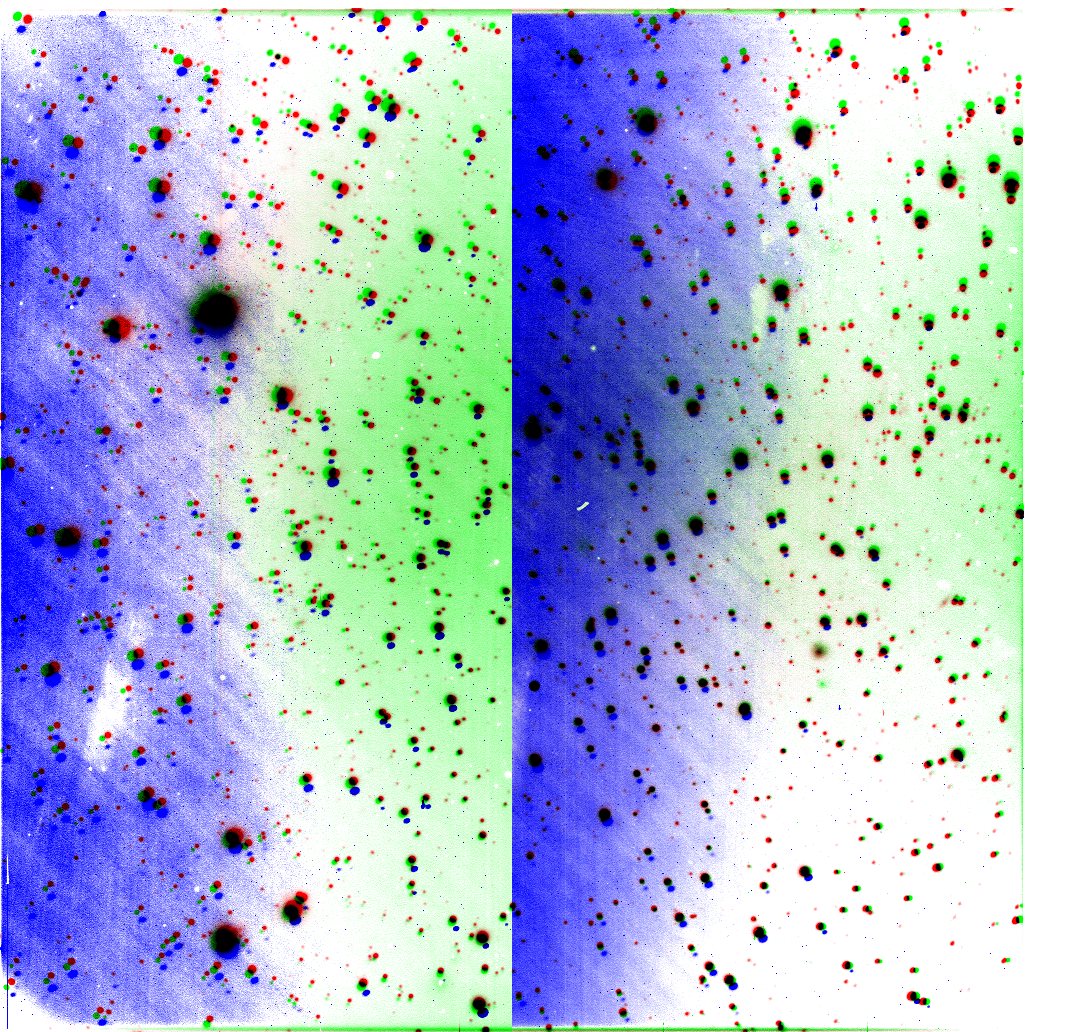
\includegraphics[width=100mm]{images/overlay_multiply.png}
  \caption{Images of the three channels overlaid (without any distortion correction applied). It is clear that the three channels do not have identical images. Translation, rotation and differential distortion are all visible. This makes matching of objects across the three channels difficult in runs with crowded fields. }
\label{fig:nonoverlap}
\end{figure}

\begin{figure}
  \centering
  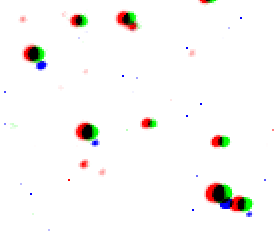
\includegraphics[width=50mm]{images/overlay_multiply_closeup.png}
  \caption{A close up of figure \ref{fig:nonoverlap} showing the bottom right hand corner. Note that the blue image is significantly translated with respect to the red and green image. To make matters worse, this distortion is not constant throughout the duration of a single run and changes with varying airmass.}
\label{fig:nonoverlapzoom}
\end{figure}

\begin{figure}
  \centering
  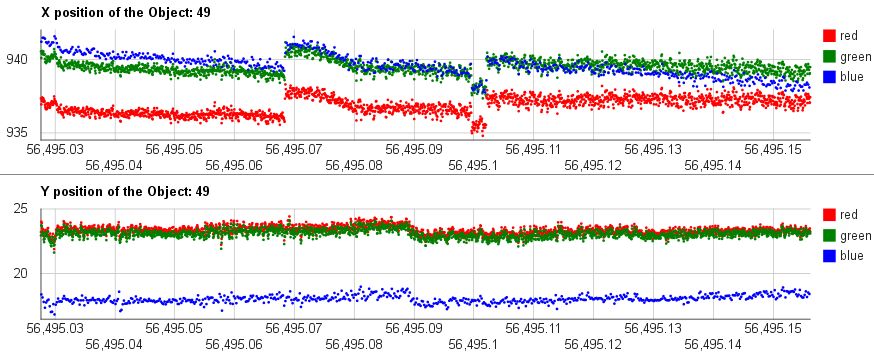
\includegraphics[width=140mm]{images/position_drift.png}
  \caption{Screen capture from the web interface showing a plot of the $(x, y)$ position of the object in the lower left corner of figure \ref{fig:nonoverlapzoom} showing how the position varies of the course of the run ($\sim 3$ hours). During this time the airmass, $\sec z$, of the target field varies from 1.02 to 1.21. Note how the $x$ position of the object in the blue channel drifts with respect to the $x$ position of the object in the red and green channels. The step changes in the object's position are caused by the observer making manual adjustments to the guiding at the telescope. }
\label{fig:positiondrift}
\end{figure}

\begin{figure}
  \centering
  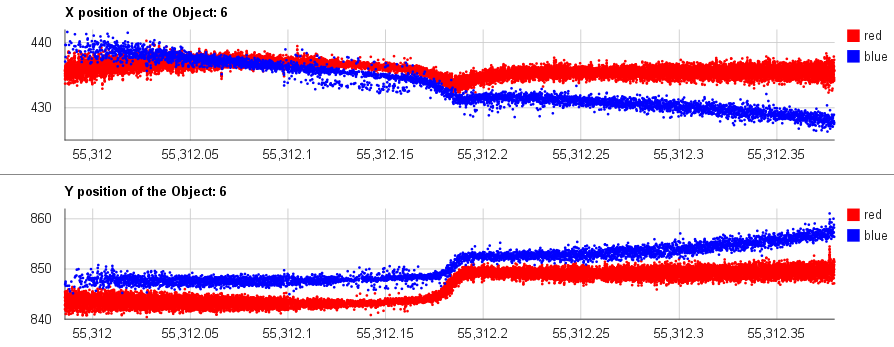
\includegraphics[width=140mm]{images/position_drift_longrun.png}
   \caption{Another screen capture from the web interface showing the change in relative positions of a single object in different channels over the course of a long run. These data are taken from the longest run in the ULTRACAM data archive, the 9.5 hour run \emph{2010-04-25/run020}. During this run, the airmass varies from a minimum of 1.0 (corresponding with the center of the plot), to a maximum of 1.99 (at the extreme left and right ends of the plot). The change in offset from the red to the blue channels is most noticeable in the $x$ position, where the blue channel's offset moves by about 13 pixels. }
\label{fig:positiondriftlongrun}
\end{figure}

Another complication is caused by the time-variation in this non-overlap of the three channels during the course of a particular observing run. When the airmass of the target field undergoes a significant change, the image distortion due to the atmosphere varies in each channel. Another factor is that the camera's physical orientation changes and the optical paths will undergo changes due to flexure in the instrument's chassis. The change in the offset position from channel to channel can be as much as 4 pixels as the airmass goes from 1.0 to 1.2 and for even larger airmass variation the object will move by as much as 13 pixels in the blue channel relative to the red and green channels. See figures \ref{fig:positiondrift} and \ref{fig:positiondriftlongrun} for examples of this drifting effect. 

The gradual movement of an object's position is dealt with in the first stage of the pipeline by allowing the object to drift gradually from frame-to-frame. It compensates by constantly updating the object's position in each frame and using the new value as the comparison position when looking for matches in the next frame. It can deal with a general slow migration in the object's position. Therefore, in the first pass of the automated pipeline, when it is building the catalogs for each channel independently of each other, it does not have problems with object matching. 

The process can fail when cross-matching across the different channels if the mean position of the object is displaced by a large amount from channel to channel, or the field is crowded and there is more than one match for any particular set of objects. Fortunately, for many of the crowded fields, an astrometric solution can be found. In this case, the pipeline  no longer relies on pixel coordinates but uses world coordinates instead to perform the match across the channels and these image distortions have been taken into account. 

Once the object cross-matching stage is complete, the pipeline writes the new three-colour master catalog to a folder on the web server, ready to be loaded by a web browser. 

% \begin{figure}
%   \centering
%   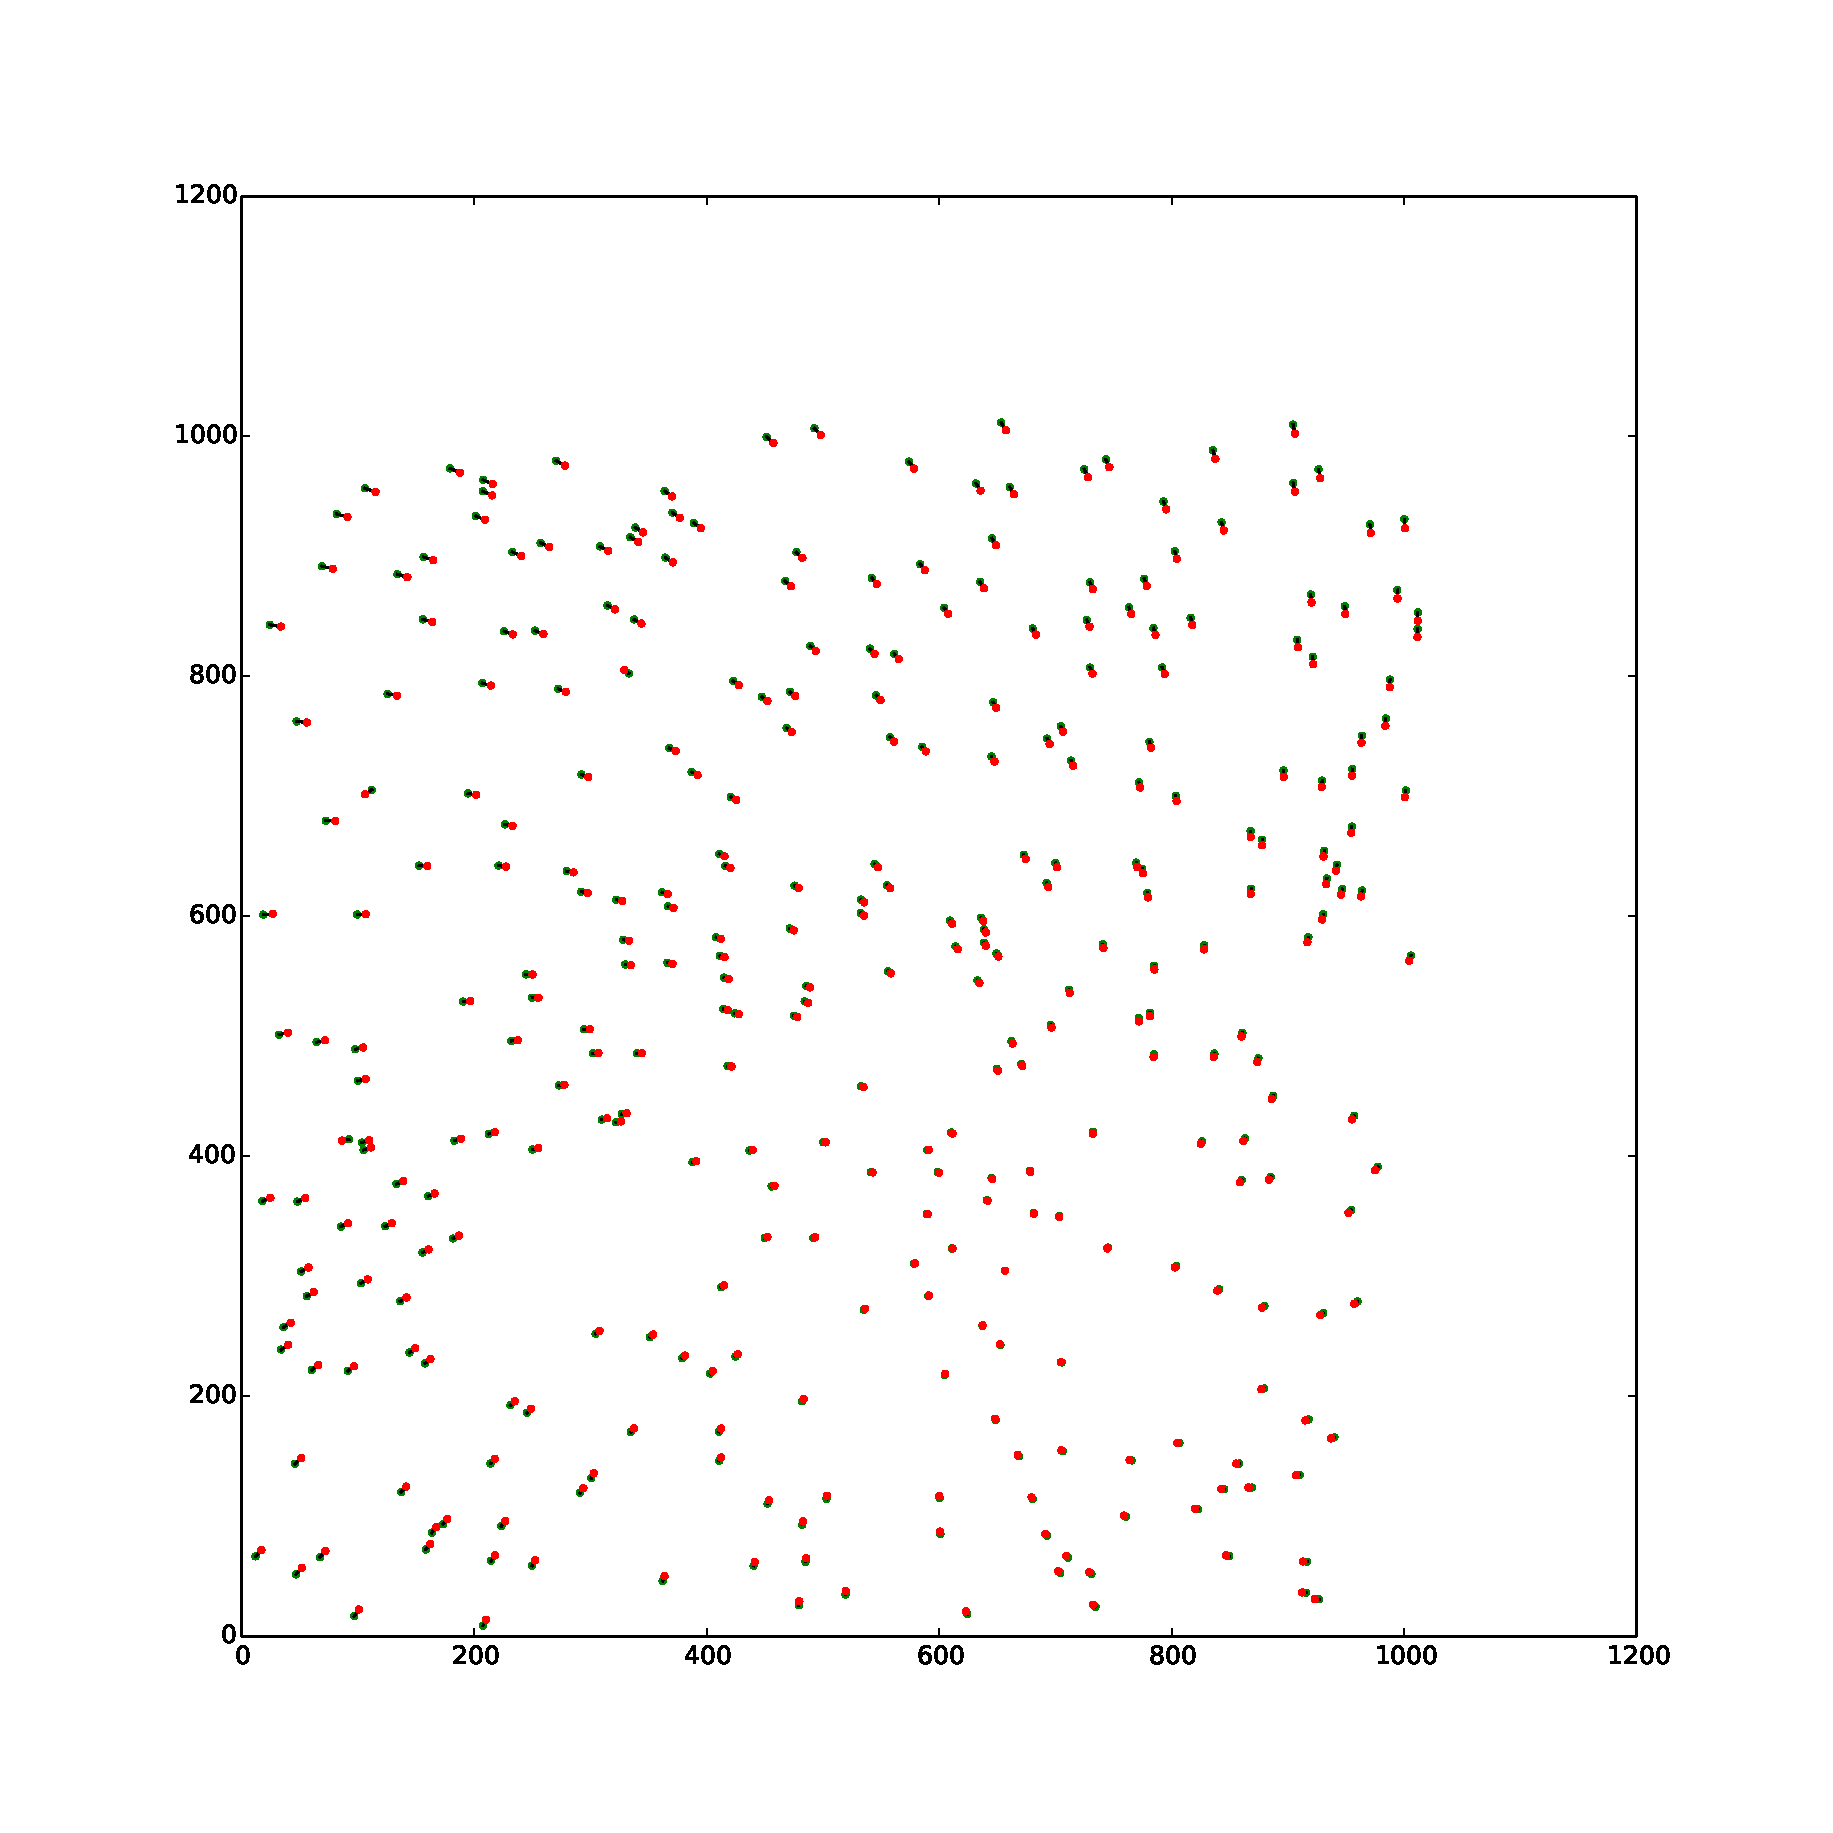
\includegraphics[width=\textwidth]{images/objectOffset_run010_g.eps}
%   \caption{The difference in object mean positions between the `red' channel and the `green' channel for run: \emph{2013-07-21/run010} }
% \label{fig:redgreenoffset}
% \end{figure}


% \begin{figure}
%   \centering
%   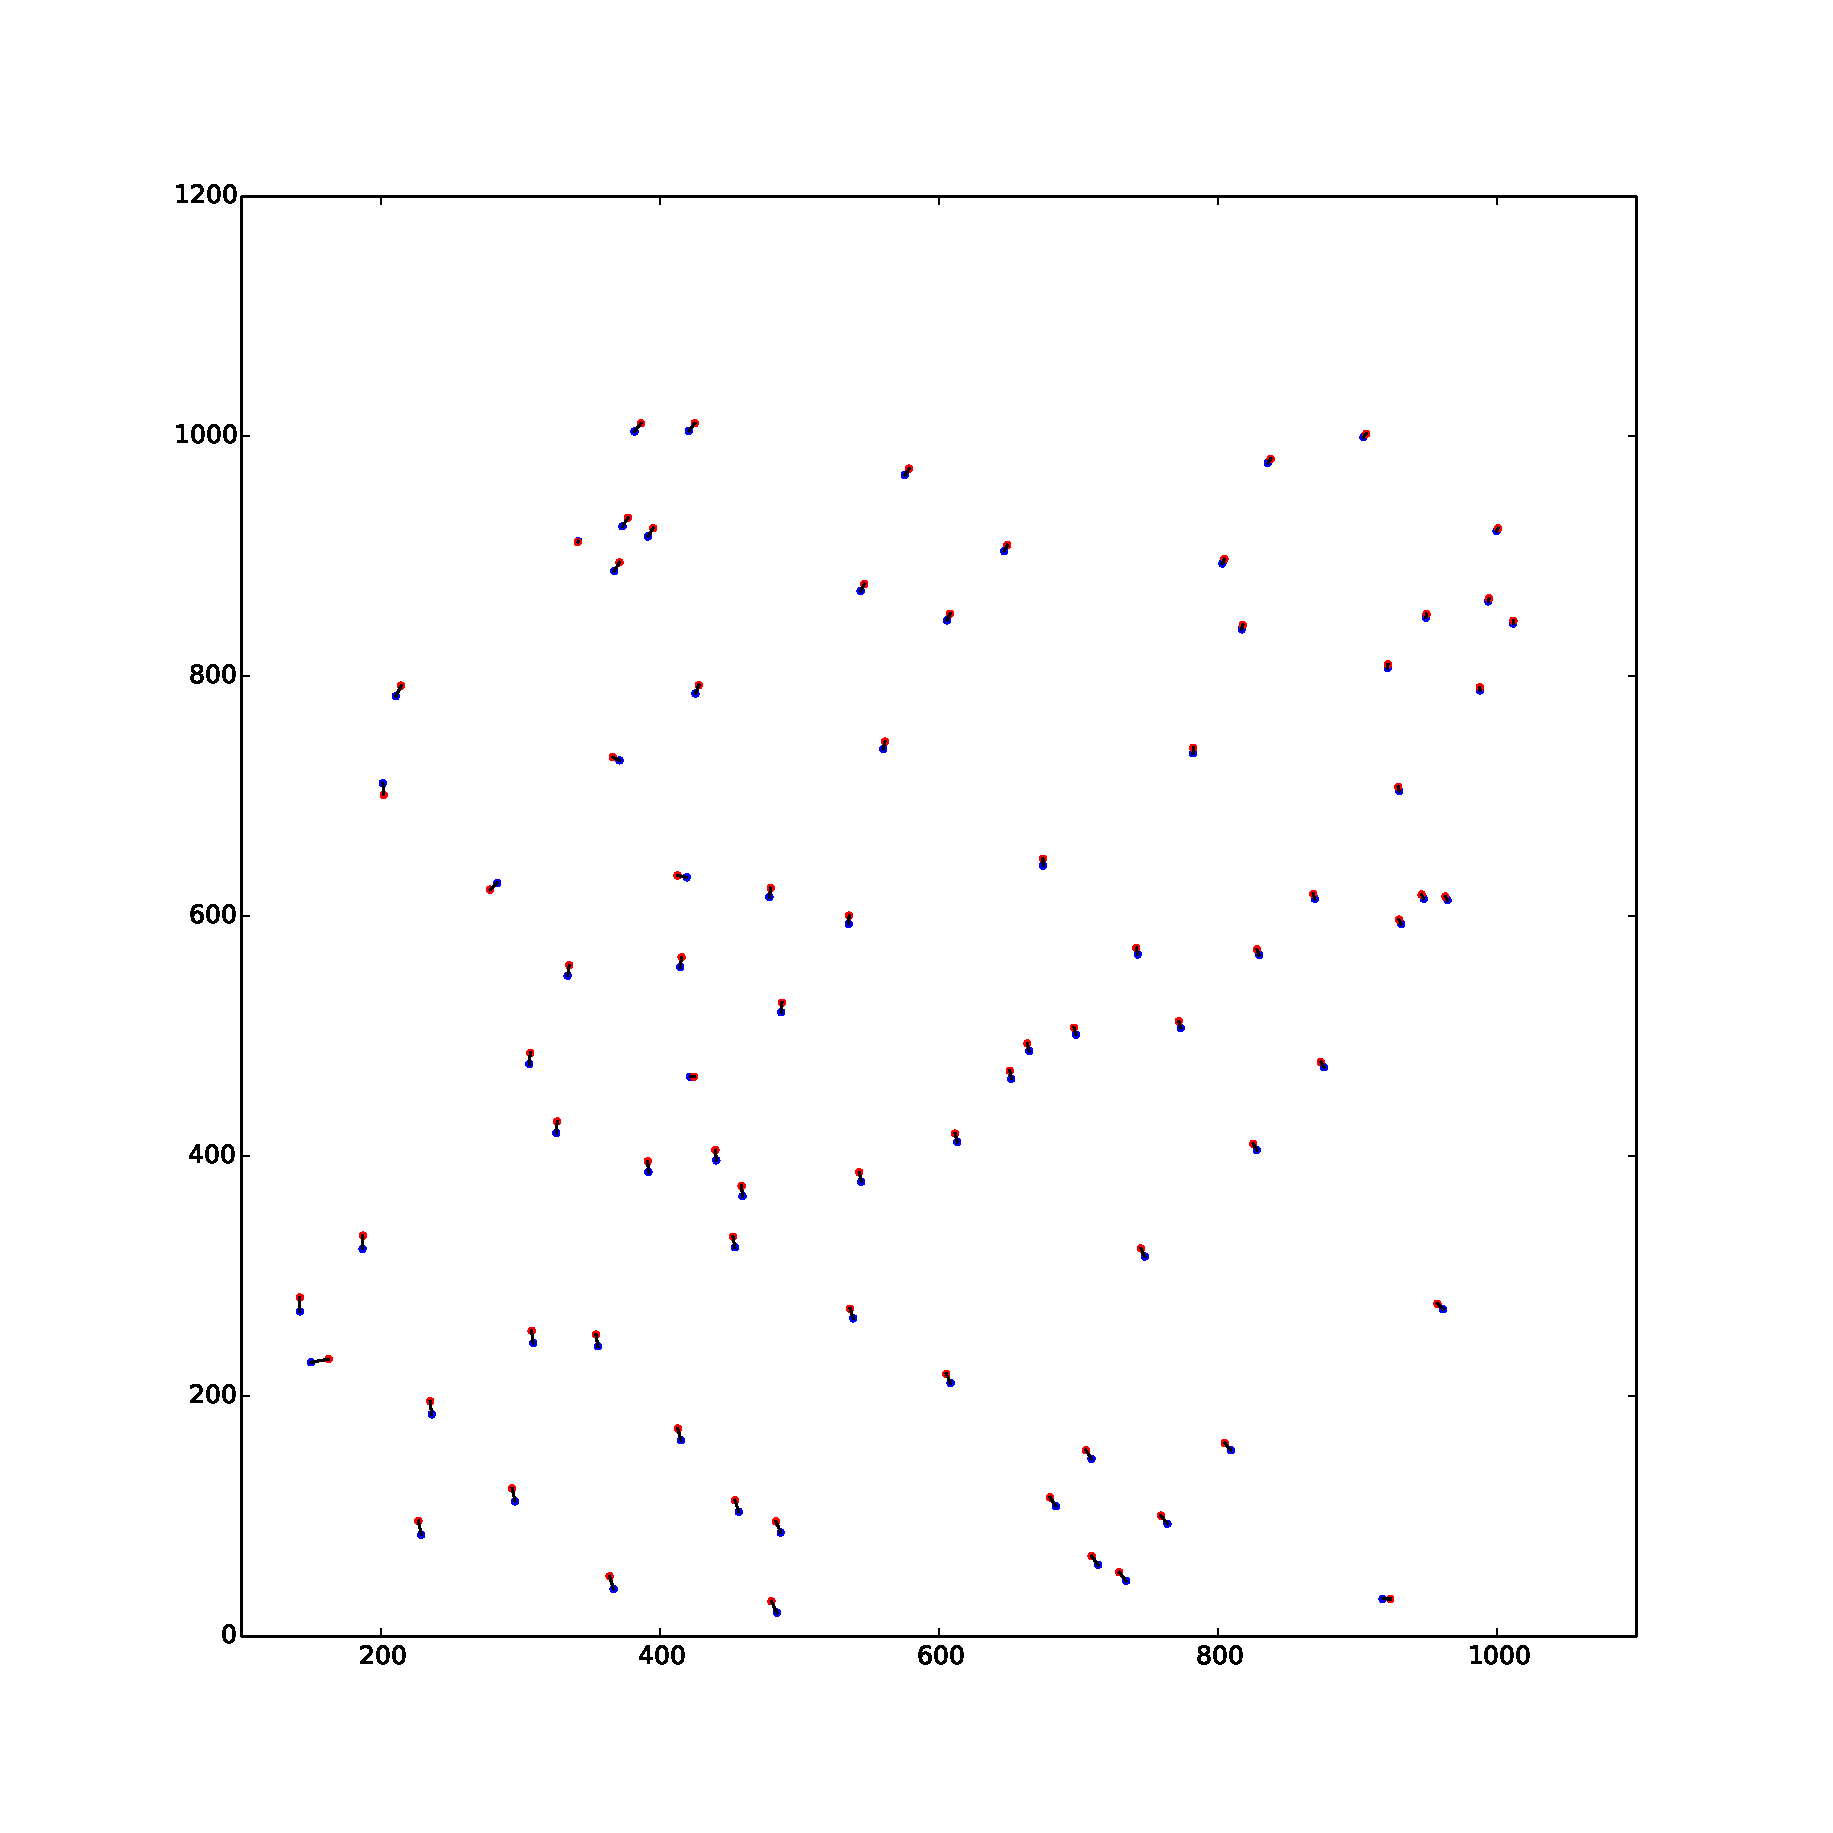
\includegraphics[width=\textwidth]{images/objectOffset_run010_b.eps}
%   \caption{The difference in object mean positions between the `red' channel and the `blue' channel for run: \emph{2013-07-21/run010} }
%   \label{fig:redblueoffset}
% \end{figure}

\subsection{WCS solutions}\label{sect:astrometry}

After tests using SCAMP \citep{scamp} and Astrometry.net \citep{astrometry} it was clear that the Astrometry.net software was more reliable at finding good WCS solutions to the fields. The software was downloaded to a local machine (including the extensive index files) and compiled. Despite being the solution that yields the most positive results so far, it still does not consistently find WCS solutions for all of the fields. There are several challenges to finding a WCS solution for the fields.

\emph{Lack of telescope pointing information}: ULTRACAM does not integrate with the telescope control software (TCS) of any of the telescopes and does not get pointing information automatically. Coordinate information relies on the observer entering a name of the candidate object for each run and then, when the data are archived, a \emph{SIMBAD} lookup is used to turn the object identifier into a right ascension and declination. This gives a world coordinate that is somewhere in the field, but it is not known which object (or pixel location) this applies to.  

\emph{Field rotation}: Since ULTRACAM can be rotated about the optical axis to allow for optimal alignment of the objects, the field of view can be at any arbitrary angle of rotation, giving an extra degree of freedom when attempting to match the field to a known catalog. 

\emph{Windows}: Many ULTRACAM runs are configured to use only portions of the CCD area. An example of this is shown in figure \ref{fig:V834Cen}. This means that there is an incomplete view of the sky for that field. When trying to match to existing indexes, there could be important, bright objects that are in the index file, but do not appear in the ULTRACAM field due to masking caused by the placement of windows on the image.

\emph{Sparse fields}: On uncrowded fields, there might have fewer than 4-5 objects to be used for field identification. 

\emph{Very small windows}: Some runs, particularly ones in high cadence mode, use very small windows (eg 172x156 pixels) in order to decrease readout time, meaning that the images (and input catalogs) might only contain two objects. This makes matching to a reference catalog impossible. 

\emph{Choice of reference index by colour}: The Astrometry.net software uses USNO-B and Tycho-2 reference catalogs by default. These are based on infra-red and V magnitudes. This means that the blue channel (which is often using the Sloan u filter) might not match the reference indexes. Indeed, current tests often result in a match in red, a match in green but no match in blue. 

After the first stage of the automated pipeline there are three catalogs of objects for each of the channels (red, green and blue). These catalogs contain pixel coordinates and flux measurements for each frame in the run that the object has been identified. The pipeline produces a simplified catalog based on the mean pixel positions and mean flux for each object $(\bar{x_i}, \bar{y_i}, \bar{F_i})$. This catalog is sorted in order of decreasing mean flux, $F$. The Astrometry.net package is given this input catalog and asked to find an astrometric solution for the field.  Astrometry.net compares objects in its reference catalog to the catalog and pixel positions in the input. The matching algorithm is based on comparing the relative positions of quadruples of stars. The indexes are derived from the USNO-B survey, which contains $\sim10^9$ stars and Tycho-2 which has $\sim2.5\times10^6$ stars. 

In addition to providing Astrometry.net with a catalog of objects to match, the pipeline also gives it the known location of the field that has been provided via a SIMBAD lookup of the coordinates of the target object as specified by the observer at the telescope. This provides the world coordinates that are guaranteed \footnote{Provided that the telescope operator has correctly entered the target name, and the SIMBAD lookup has been successful.} to be somewhere within the field. The pipeline provides a limit to the coordinates of the solution as a maximum distance of 1 degree from the input location. It also provides upper and lower limits to the expected field scale of the solution. Providing these parameters saves computation time as it restricts Astrometry.net to a small region of the potential solution space and removes the need for doing a comprehensive search. Considering that the field sizes are only a few arc minutes wide, specifying 1 degree as the search radius is probably overkill. A future task for this automated pipeline project will be to find the optimal value for this parameter.

\begin{figure}
  \centering
  \includegraphics[width=\textwidth]{images/sip_correction_r_10x.eps}
  \caption{The SIP polynomial fit of the WCS solution for the red channel of run \emph{2013-07-21/run010}. The vectors were computed by transforming from pixel coordinates to world coordinates first without the SIP polynomial, then doing the same transformation with the SIP polynomial. The lengths of the vectors have been multiplied by $10\times$.}
\label{fig:sipred}
\end{figure}

\begin{figure}
  \centering
  \includegraphics[width=\textwidth]{images/sip_correction_g_5x.eps}
  \caption{The SIP polynomial fit of the WCS solution for the green channel of run \emph{2013-07-21/run010}. The vectors were computed by transforming from pixel coordinates to world coordinates first without the SIP polynomial, then doing the same transformation with the SIP polynomial. The lengths of the vectors have been multiplied by $5\times$.}
\label{fig:sipgreen}
\end{figure}

\begin{figure}
  \centering
  \includegraphics[width=\textwidth]{images/sip_correction_b_10x.eps}
  \caption{The SIP polynomial fit of the WCS solution for the red channel of run \emph{2013-07-21/run010}. The vectors were computed by transforming from pixel coordinates to world coordinates first without the SIP polynomial, then doing the same transformation with the SIP polynomial. The lengths of the vectors have been multiplied by $10\times$.}
\label{fig:sipblue}
\end{figure}

If Astrometry.net can find a solution for the field, it generates a FITS format file containing the parameters defining the solution. These parameters consist of the position in right ascension and declination $(\alpha_{ref}, \delta_{ref})$ of a particular reference pixel in the image $(x_{ref}, y_{ref})$, plus 4 parameters that define a transformation matrix to move from pixel coordinates $(x, y)$ to world coordinates, $(\alpha, \delta)$. These values are labeled $CD1\_1$, $CD1\_2$, $CD2\_1$ and $CD2\_2$. The transformation from pixel coordinates to world coordinates is given by: \begin{equation} 
\left(\begin{array}{c} \alpha \\ \delta \end{array} \right) = \left(\begin{array}{c} \alpha_{ref} \\ \delta_{ref} \end{array} \right) + 
\left(\begin{array}{cc}  CD1\_1 & CD1\_2 \\ CD2\_1  & CD2\_2 \\ \end{array}\right) 
\left(\begin{array}{c} x' \\ y' \end{array} \right)
\end{equation}
Where $(x', y')$ are the pixel offsets to the reference pixel $(x_{ref}, y_{ref})$.

\begin{figure}
  \centering
  \includegraphics[width=\textwidth]{images/greentored.eps}
  \caption{An indication of the difference in the images from channel to channel,  comparing the green to the red channel. The background image shows the deep image of the field. The vectors leading away from the objects were generated by calculating the world coordinates (WCS) for the object's position with the green WCS solution and then reverting them back to pixel coordinates using the red WCS solution. The lengths of the vectors have been exaggerated on this image by a factor of 2. The median vector length is 5.7 pixels }
\label{fig:greentored}
\end{figure}
  
\begin{figure}
  \centering
  \includegraphics[width=\textwidth]{images/bluetored.eps}
  \caption{An indication of the difference in the images from channel to channel, comparing the blue to the red channel. The background image shows the deep image of the field. The vectors leading away from the objects were generated by calculating the world coordinates (WCS) for the object's position with the blue WCS solution and then reverting them back to pixel coordinates using the red WCS solution. The lengths of the vectors have been exaggerated on this image by a factor of 2. The median vector length is 9.4 pixels.}
\label{fig:bluetored}
\end{figure}

The four transformation values $(CD1\_1, CD1\_2, CD2\_1, CD2\_2)$, define a scale transformation and a rotation from pixel to world coordinates. They do not express distortion across the image. In order to encapsulate this distortion, Astrometry.net also provides Simple Imaging Polynomial (SIP) correction parameters, \citep{sippolynomial}. For this project, a SIP polynomial of the 3rd order is used to account for distortion across the ULTRACAM field. The correcting factors provided by the SIP polynomial are generally small, providing a corrections of a few tenths to one pixel. The extent to which the these non-linear distortion terms affect the image is shown in figures \ref{fig:sipred}, \ref{fig:sipgreen} and \ref{fig:sipblue}. 

Since each channel has its own WCS solution, comparing these across the three channels gives an indication of the difference of the image from channel to channel. Figures \ref{fig:greentored} and \ref{fig:bluetored} show the difference in the green and blue WCS solutions for each object in the field relative to the WCS solution in the red field (for the run \emph{2013-07-21/run010}). The shifts were computed by taking the pixel coordinates of each object, transforming them into world-coordinates using the WCS solution specific to that channel and then converting back to pixel coordinates via the WCS solution for the red channel. The difference in these pixel coordinates shows how the distortion varies across the image.  For the run, \emph{2013-07-21/run010} the median separation is 5.7 pixels in the green channel and 9.4 pixels in the blue channel. 

The parameters defining the WCS solutions are saved to the web repository as a JSON\footnote{Javascript Object Notation (JSON) is a plain text file format that encapsulates object structure and is becoming a increasingly common way to store data to be displayed on web pages. It has some similarities to XML, but with a reduced syntax. It is described in more detail in the following chapter \ref{chap:webfrontend}.} object, ready to be loaded when the web browser accesses the page. 

\section{Summary}
At this stage of the pipeline, the bulk of the data reduction work is complete and the results are ready to be staged for rendering on the web. The next chapter will describe how this information is made available through a web site such that it can be accessed and viewed in a web-browser. 
